\section{Experiment 2: Analyzing Fairness between TCP Variants}

This experiment used two TCP flows and a single CBR flow, to analyze the fairness between the TCP flows among different pairs of TCP variants. We tested different combinations of variants, including assigning TCP Vegas to both flows, TCP Reno to both flows, NewReno to one flow and Reno to another, and NewReno to one flow and Vegas to another. Further, we ran two slightly different simulations. The first simulation analyzes fairness in a network with a CBR flow rate of 1 Mbps and an initial packet size of 1000 bytes. The second simulation analyzes fairness is a network with a CBR flow rate of 10 Mbps and an initial packet size of 10,000 bytes. The first test simulates a network with little-to-no congestion, and the second test simulates a network with high congestion and packet loss.

\subsection{Simulation 1: Little-to-No Network Congestion}

In the network with no congestion, the throughputs of the individual streams given the combinations of Reno/Reno and NewReno/Reno were all equal, at .56 Mbps. This is to be expected. There were no packet losses, therefore NewReno stream acted as a Reno stream. This is because the variants only differ in what they do after multiple packet drops. After the first packet drop, both variants use fast retransmit and inflate their congestion windows to allow for outstanding packets between the source and destination to complete their transmissions. 

The throughputs of the two Vegas streams, were .55 and .6 Mbps. This can be a result of one stream calculating a higher than expected RTT and reducing the congestion window, allowing the other to maintain and increase the cwnd size. Unlike Reno and NewReno, Vegas is not deterministic given no packet drops. The largest discrepancy between any two streams we tested, was that of NewReno and Vegas. The average throughput of NewReno was .98 Mbps, and the throughput of Vegas was .15 Mpbs. The average latencies of each pair of variants in this low congestion network, were very close.

TCP Vegas senses congestion through larger than expected RTT values, and proceeds to decrease its congestion window. TCP NewReno continuously increases its window size until loss actually occurs. Even though there were no packet drops and little to no congestion, the aggressive nature of TCP NewReno monopolizes the bandwidth of the streams, reducing the throughput of the more cautious TCP Vegas.

\subsection{Simulation 2: High Network Congestion}

Each combination of variants in the second simulation saw high amounts of congestion. This simulation consisted of a CBR flow with a rate of 10 Mbps and initialized all packet sizes to 10,000 bytes. Although the combination of TCP Vegas, once again resulted in similar throughputs for individual streams - at about .1 Mbps each, we note that these throughputs are much smaller than what was scene in the previous simulation. The throughput was much lower because each stream sensed the congestion caused by the other flow; however, there were no packet drops, instead the congestion window was continuously decreased. The combination of Reno/Reno also saw lower, but equal throughputs, with each stream maintaining an average throughput of about .2 Mbps. In this case, we saw 23 packet drops. Still, the fast recovery and fast retransmit process is the same for both of these streams, so the similar throughputs are to be expected.

The combination of NewReno/Reno resulted in a larger throughput discrepancy given the congested network. NewReno, as expected achieved the slightly higher throughput of .23 Mbps where as Reno's throughput was .185 Mbps. There were 30 total packets dropped. If the simulation had run for longer, we predict the number of dropped packets would increase and the discrepancy between the throughputs of the NewReno and Reno streams would grow even larger. FIgure 4 depicts the number of dropped packets for each variant when combined with another.

\begin{figure}[!htbp]
	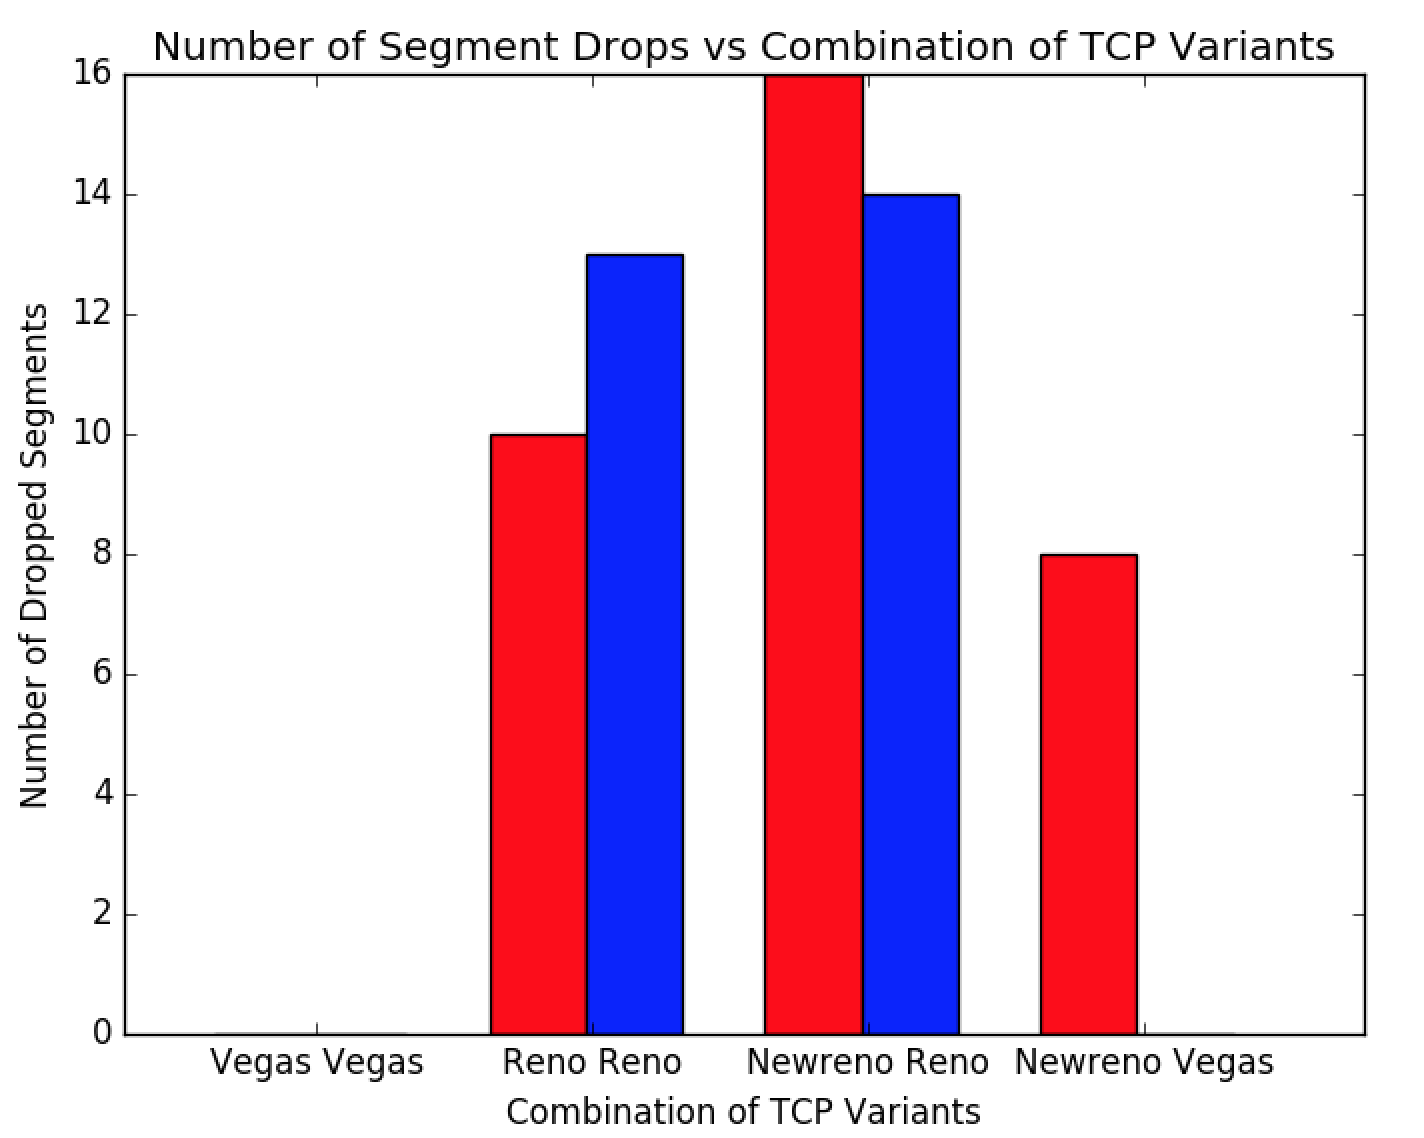
\includegraphics[scale=0.3]{exp2_dp.png}
	\caption{This figure depicts the number of segments dropped for each variant, when sharing bandwidth with another TCP stream.}
	\label{a:label}
\end{figure}


Despite the fact that both Reno and NewReno inflate their congestion window size by the number of duplicate acknowledgments, Reno requires any additional packet losses to be detected by the retrasmission timeouts or 3 duplicate acknowledgments. NewReno retransmits lost packets more efficiently by assuming that the next partial acknowledgement marks a lost packet which is immediately retransmitted. The increased throughput of NewReno is a direct result of this assumption. Ultimately both Reno and NewReno deflate their congestion windows, but only after outstanding packets have been properly acknowledged by the receiver.

This discrepancy is more dramatic when assigning one stream to TCP NewReno and another to TCP Vegas. NewReno had an average throughput of .26 Mpbs and Vegas at .1 Mpbs. Only 8 packets were dropped in this simulation, all by the TCP NewReno stream. NewReno utilizes an increasing amount of the link before and in the immediate aftermath of a packet loss occur. Vegas, on the other hand, continuously decreases its congestion window as it perceives the increased utilization by NewReno, as congestion. However, we notice the discrepancy in throughputs here, is not as large as the discrepancy we saw in the first simulation. This is because the packets dropped by NewReno, although inflating the congestion window initially, ultimately deflated the window, reducing the size of the packets being released into the network. The throughputs of each stream on the shared network are depicted in Figure 5.

\begin{figure}[!htbp]
	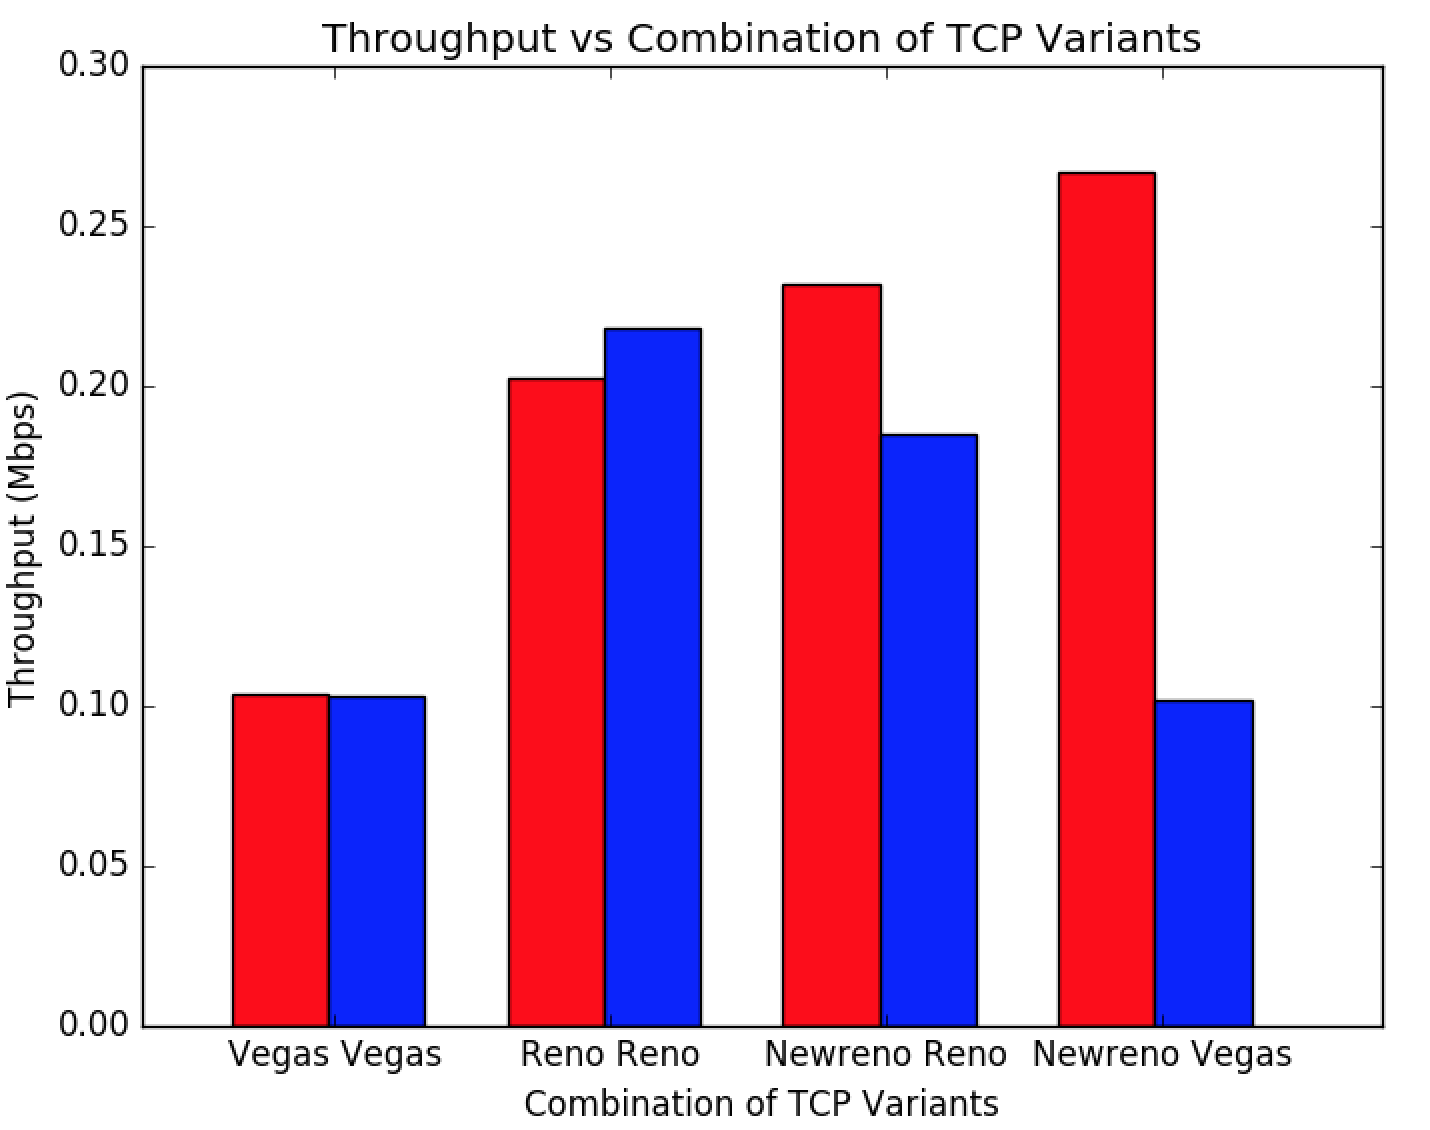
\includegraphics[scale=0.3]{exp2_tp.png}
	\caption{This figure depicts the throughput for each variant, when sharing bandwidth with another TCP stream.}
	\label{a:label}
\end{figure}



